\documentclass{article}

\usepackage{fancyhdr}
\usepackage{lastpage}
\usepackage{extramarks}
\usepackage[usenames,dvipsnames]{color}
\usepackage{courier}
\usepackage{amsmath}
\usepackage{amsthm}
\usepackage{amsfonts}
\usepackage{tikz}

\usetikzlibrary{automata,positioning}

\topmargin=-0.45in
\evensidemargin=0in
\oddsidemargin=0in
\textwidth=6.5in
\textheight=9.0in
\headsep=0.25in

\linespread{1.1}

\pagestyle{fancy}
\lhead{\hmwkAuthorName}
\chead{\hmwkClass\ (\hmwkClassInstructor\ \hmwkClassTime): \hmwkTitle}
\rhead{\firstxmark}
\lfoot{\lastxmark}
\cfoot{}
\renewcommand\headrulewidth{0.4pt}
\renewcommand\footrulewidth{0.4pt}

\setlength\parindent{0pt}

\newcommand{\enterProblemHeader}[1]{
    \nobreak\extramarks{#1}{#1 continued on next page\ldots}\nobreak
    \nobreak\extramarks{#1 (continued)}{#1 continued on next page\ldots}\nobreak
}

\newcommand{\exitProblemHeader}[1]{
    \nobreak\extramarks{#1 (continued)}{#1 continued on next page\ldots}\nobreak
    \nobreak\extramarks{#1}{}\nobreak
}

\setcounter{secnumdepth}{0}
\newcounter{homeworkProblemCounter}

\newcommand{\homeworkProblemName}{}
\newenvironment{homeworkProblem}[1][Problem \arabic{homeworkProblemCounter}]{
    \stepcounter{homeworkProblemCounter}
    \renewcommand{\homeworkProblemName}{#1}
    \section{\homeworkProblemName}
    \enterProblemHeader{\homeworkProblemName}
}{
    \exitProblemHeader{\homeworkProblemName}
}

\newcommand{\problemAnswer}[1]{
    \noindent\framebox[\columnwidth][c]{\begin{minipage}{0.98\columnwidth}#1\end{minipage}}
}

\newcommand{\homeworkSectionName}{}
\newenvironment{homeworkSection}[1]{
    \renewcommand{\homeworkSectionName}{#1}
    \subsection{\homeworkSectionName}
    \enterProblemHeader{\homeworkProblemName\ [\homeworkSectionName]}
}{
    \enterProblemHeader{\homeworkProblemName}
}

\newcommand{\hmwkTitle}{Homework\ \#3}
\newcommand{\hmwkDueDate}{February 14, 2013 at 11:59pm}
\newcommand{\hmwkClass}{CS331}
\newcommand{\hmwkClassTime}{9:00am}
\newcommand{\hmwkClassInstructor}{Professor Zhang}
\newcommand{\hmwkAuthorName}{Josh Davis}

\title{
    \vspace{2in}
    \textmd{\textbf{\hmwkClass:\ \hmwkTitle}}\\
    \normalsize\vspace{0.1in}\small{Due\ on\ \hmwkDueDate}\\
    \vspace{0.1in}\large{\textit{\hmwkClassInstructor\ \hmwkClassTime}}
    \vspace{3in}
}

\author{\textbf{\hmwkAuthorName}}
\date{}

\begin{document}

\maketitle

\pagebreak

\begin{homeworkProblem}
    Prove that if \(L\) is regular, then so is \(L_{\frac{1}{2}}\).
    
    \begin{proof}
        We will show that if \(L\) is regular, then so is \(L_{\frac{1}{2}}\).
        \\
    
        Suppose that \(L\) is regular. Since \(L\) is regular, that means we
        can create a automata for it. Let this automata be \(A\) such that
        \(L(A) = L\). Also let B be an automata such that \(L(B) = L^R\). The
        automata can also be defined as follows:
        \[
            \begin{split}
                A = (Q_A, \Sigma, \delta_A, q_{A}, F_A)
                \\
                B = (Q_B, \Sigma, \delta_B, q_{B}, F_B)
            \end{split}
        \]
        
        
        Since \(L\) is regular, we know that \(L^R\) is also regular because of
        homework two from last week.
        \\

        Now we will make an automata \(C\) constructed from \(A\) and \(B\).
        This will show that \(L_{\frac{1}{2}}\) is regular. \(C\) will be
        defined as follows:

        \[
            C = (Q, \Sigma, \delta, q, F)
        \]

        where

        \begin{enumerate}
            \item \(Q = Q_A \times Q_B\) 
            \item The alphabet is the same, \(\Sigma = \Sigma\)
            \item The start is in the start state for \(A\) and the ending
            state of \(B\), \(q = (q_A, F_B)\).
            \item The final is when we are at the end of \(A\) but the start of
            \(B\), \(F = (F_A, q_B)\)
            \item Define \(\delta\) so that
            \[
                \delta((q_1, q_2), a) = \left\{
                    \begin{array}{ll}
                        (\delta_A(a), q_2) & \quad a \in w \\
                        (q_1, \delta_B(a)) & \quad a \in w'
                    \end{array}
                \right.
            \]
            where \(w \in L\) such that \(\left|w\right| = \left|w'\right|\) and \(ww' \in L\).
        \end{enumerate}

        The reason this works is because we just create an automata that is the
        cross product of both of their states. Therefore we create a grid of
        states such that \(q_1 \in Q_A\) and \(q_2 \in Q_B\). Then if we just
        start at the beginning of \(A\) and the end of \(B\) then only
        accept it when we reach the end of both strings, then it is a valid automata
        that satisfies the condition.

    \end{proof}

\end{homeworkProblem}

\pagebreak

\begin{homeworkProblem}
\end{homeworkProblem}

\begin{homeworkProblem}
    Prove that the language \(L\) such that "w is not a palindrome" is not regular.
    \begin{proof}
        We will show \(L\) is irregular by showing that the complement of \(L\), \(L'\) or "w is a palindrome"
        is regular. This is valid because languages are closed under the complement.
        \\

        Let \(w = 0^{p}10^{p}\) which is a palindrome and in \(L'\). Now assume that \(L'\) is regular.
        According to the pumping lemma, \(w = xyz\) and let \(p\) be the
        pumping length. Without taking the third condition of the pumping lemma into
        consideration gives us six cases for splitting \(w\).

        \begin{enumerate}
            \item The string y consists of all 0s at the beginning of \(w\).
            \item The string y consists of 01s.
            \item The string y consists of 10s.
            \item The string y consists of all 1s.
            \item The string y consists of all 0s at the end of \(w\).
            \item The string y consists of 010s.
        \end{enumerate}

        The cases of 2, 3, 4, 5, 6  all violate the third condition of the pumping
        lemma, that \(\left|xy\right| \leq p\). Therefore we have cornered
        \(y\) and are only left with case 1.
        \\

        Now we can pump \(y\) which gives us more 0s at the beginning of \(w\)
        than at the end. Therefore \(w\) is no longer a palindrome and thus not
        in \(L\). We have arrived at a contradiction which shows that the
        language \(L'\) is not regular. Therefore the complement of \(L'\) is
        just \(L\) and also not regular.
    \end{proof}
\end{homeworkProblem}

\pagebreak

\begin{homeworkProblem}
    Let \(k > 1\), \(L_k = \{\epsilon, a, aa, \dots, a^{k - 2}\}\)
    \begin{proof}
        \textbf{Part 1}
        \\

        \(L_k\) can be recognized by a DFA with k states. To show this, we will
        construct a DFA as follows:

        \begin{figure}[here]
            \centering
            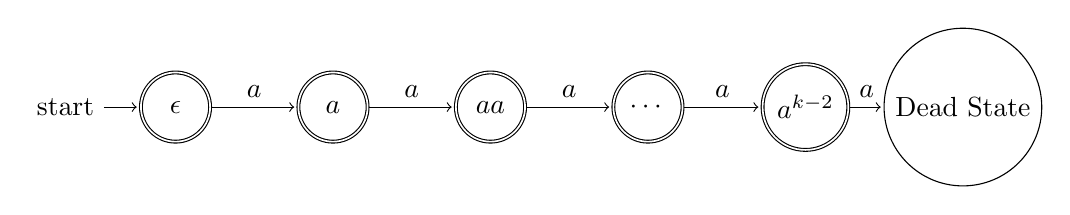
\begin{tikzpicture}[shorten >=1pt,node distance=2cm,on grid,auto] 
                \node[state, initial, accepting] (a_0) {$\epsilon$}; 
                \node[state, accepting] (a) [right=of a_0] {$a$}; 
                \node[state, accepting] (aa) [right=of a] {$aa$}; 
                \node[state, accepting] (a_dots) [right=of aa] {$\cdots$}; 
                \node[state, accepting] (a_{k-2}) [right=of a_dots] {$a^{k-2}$}; 
                \node[state] (dead) [right=of a_{k-2}] {Dead State}; 
                \path[->] 
                    (a_0)
                        edge node {$a$} (a)
                    (a)
                        edge node {$a$} (aa)
                    (aa)
                        edge node {$a$} (a_dots)
                    (a_dots)
                        edge node {$a$} (a_{k-2})
                    (a_{k-2})
                        edge node {$a$} (dead);
            \end{tikzpicture}
            \caption{DFA, \(A\)}
            \label{fig:automataA}
        \end{figure}

        As we can see, there will be one starting state, \(k-2\) additional
        states, and then one dead state. Therefore there are \(1 + (k-2) + 1 = k\) states.

        \textbf{Part 2}
        \\


    \end{proof}
\end{homeworkProblem}

\pagebreak

\begin{homeworkProblem}
    Co-determinism.

    \begin{proof}
        \textbf{Show that every CDFA is a DFA.}
        \\

        To do this, we will look at what the differences are between a DFA and
        NFA. A NFA has the following differences:
        \begin{enumerate}
            \item Alphabet = \(\Sigma_{\epsilon}\), allows epsilon transitions
            \item Can have 0 or more transitions for any given input and state
        \end{enumerate}

        A CDFA has already been defined for us. Therefore it has these
        differences from a NFA:
        \begin{enumerate}
            \item Allows only input from \(\Sigma\), no epsilon
            \item Cannot have multiple transitions with the same input going
            into the same state, or \(\delta(q, a) \cap \delta(q', a) =
            \emptyset\)
        \end{enumerate}

        It can be seen that a CDFA and NFA do not share the same properties.
        Therefore a CDFA is just a more specific DFA.
    \end{proof}

    \textbf{Show that every DFA is a CDFA.}
    \\

    \textbf{Counterexample} To show that this is not true, we can take the given
    DFA:
    \begin{figure}[here]
        \centering
        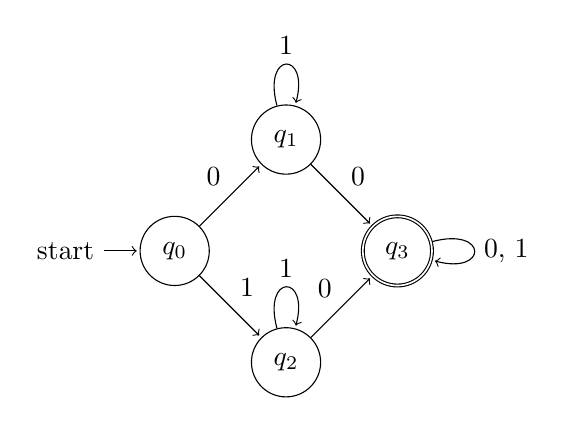
\begin{tikzpicture}[shorten >=1pt,node distance=2cm,on grid,auto] 
            \node[state, initial] (q_0) {$q_0$}; 
            \node[state] (q_1) [above right=of q_0] {$q_1$}; 
            \node[state] (q_2) [below right=of q_0] {$q_2$}; 
            \node[state, accepting] (q_3) [above right=of q_2] {$q_3$}; 
            \path[->] 
                (q_0)
                    edge node {0} (q_1)
                    edge node {1} (q_2)
                (q_1)
                    edge [loop above] node {1} ()
                    edge node {0} (q_3)
                (q_2)
                    edge [loop above] node {1} ()
                    edge node {0} (q_3)
                (q_3)
                    edge [loop right] node {0, 1} ();
        \end{tikzpicture}
        \caption{NFA, \(B\)}
        \label{fig:counterexample1}
    \end{figure}

    The Figure~\ref{fig:counterexample1} is a counterexample because it has
    a state, \(q_3\), that has two incoming arrows for state 0. Thus it violates
    the definition of co-determinism.

    \begin{proof}
        \textbf{Show that every NFA can be converted into an equivalent CDFA.}
        \\\\
        Using the theorem 1.39 out of Sipser's book, it is proven that every NFA
        can be converted into an equivalent DFA.
        \\

        Taking that same DFA, one could add more states to (maximizing) it and
        it would be possible to reduce all same input transisitions to a single
        state down to none such that
        \(\delta(q, a) \cap \delta(q', a) = \emptyset\).
        \\

        Once this has been achieved, the state machine would then be
        co-deterministic.
    \end{proof}
\end{homeworkProblem}

\end{document}
